\documentclass[a4paper,12pt]{scrartcl}

\usepackage[utf8]{inputenc}
\usepackage[T1]{fontenc}
\usepackage{amsmath}
\usepackage[ngerman]{babel}
\usepackage[a4paper,margin=1.5cm]{geometry}
\usepackage{tikz}
\usepackage{circuitikz}
\usetikzlibrary{calc, positioning}
\usepackage{booktabs}
\usepackage{xcolor}
\usepackage[automark,headsepline,footsepline]{scrlayer-scrpage}



\title{Formelsammlung GET 2 2026}
%\subtitle{text}
\author{}
%\date{\today}

% Dunkelgrün definieren
\definecolor{darkgreen}{rgb}{0.0,0.5,0.0}

% TikZ Stil für Hinweispfeile
\tikzset{
  hint/.style={->, >=latex, thick, darkgreen}
}

% Einheitliche Zeilenhöhe in Tabellen mit array Paket
\usepackage{array}
\renewcommand{\arraystretch}{1.5}

\begin{document}



\begin{center}
%\maketitle
\end{center}

\section{Foliensatz 1}

%\clearpairofpagestyles
%\ihead{\rightmark}
%\ohead{\leftmark}
%\ofoot{Stand: \today}
%\cfoot{\pagemark}

\begin{tabular}{@{} l l @{}}

Wechselspannungen \\
\hspace*{20mm} Kreisfrequenz & $\omega = \dfrac{2 \pi}{T} = 2 \pi f$ \\
\hspace*{20mm} Frequenz & $f = \dfrac{1}{T} = \dfrac{\omega}{2 \pi}$ \\

\hspace{20mm} arithmetisches Mittel & $\overline{U}=\dfrac{1}{T}\int_0^T U(t) dt$ \\
\hspace*{20mm} Effektivwert & $U_{eff} = \sqrt{\dfrac{1}{T}\int_0^T U^2(t) dt}$ \\
 & $\Rightarrow U_{eff} = \dfrac{U_0}{\sqrt{2}}$ für Harmonische Signale \\

 \hspace{20mm} Gleichrichtwert & $U_{gl} = \dfrac{1}{T}\int_0^T |U(t)| dt$ \\

 \hspace*{20mm}Harmonische Wechselspannung über Zeit& $U(t) = \sqrt{2} \cdot U \cdot \cos(\omega t + \varphi_u)= \sqrt{2} \cdot Re(\underline{U} \cdot e^{j\omega t})$ \\
 \hspace*{20mm}Phasor & $\underline{U} = {U_0} \cdot e^{j\varphi_u}$ \\
Komplexe Zahlen \\
\hspace{20mm}Euler Theorem & $e^{j\varphi} = \cos(\varphi) + j \sin(\varphi)$ \\
& $j=\sqrt{-1} \Rightarrow j^2 = -1$ \\
\hspace{20mm} Realteil komplexer Zahl $e^{jx}$ & $Re(e^{jx}) = \cos(x)$ \\
\hspace*{20mm} Imaginärteil komplexer Zahl $e^{jx}$ & $Im(e^{jx}) = \sin(x)$ \\
\hspace*{20mm} Kehrwert komplexer Zahl & $\dfrac{1}{j}=-j$ \\
\hspace*{20mm} Konjugiert komplexe Erweiterung & $\dfrac{1}{a+jb} = \dfrac{a}{a^2+b^2} + j \cdot \dfrac{(-b)}{a^2+b^2}$ \\
Komplex Bauteilgestze \\
\hspace*{20mm} Spule & $U = L \cdot \dfrac{dI}{dt} \Rightarrow \underline{U} = j\omega L \cdot \underline{I}$ \\
\hspace{20mm} Kondensator & $I = C \cdot \dfrac{dU}{dt} \Rightarrow \underline{I} = j\omega C \cdot \underline{U}$ \\
\hspace*{20mm} Widerstand & $U = R \cdot I \Rightarrow \underline{U} = R \cdot \underline{I}$ \\
\hspace*{20mm} Impedanz & $\underline{U} = \underline{Z} \cdot \underline{I}$ \\
 & $\underline{Z} = j\omega L$ für Spule \\
  & $\underline{Z} = \dfrac{1}{j\omega C}$ für Kondensator \\
  & $\underline{Z} = R$ für Widerstand \\

komplexer Widerstand & $\underline{Z} = R + jX$ \\
\hspace*{20mm} Realteil & $Re(\underline{Z}) $ Wirkwiderstand \\
\hspace*{20mm} Imaginärteil & $Im(\underline{Z})$ Blindwiderstand (Reaktanz)\\
\hspace*{20mm} Kondensator & $Im(\underline{Z}) = -\dfrac{1}{\omega C}$ \\
\hspace*{20mm} Spule & $Im(\underline{Z}) = \omega L$ \\

\end{tabular}

\newpage
\subsection{Koordinaten umformen}
\begin{figure}[h] % [h] versucht das Bild genau HIER zu platzieren
    \centering
    % width=0.5\textwidth macht das Bild halb so breit wie den Text
    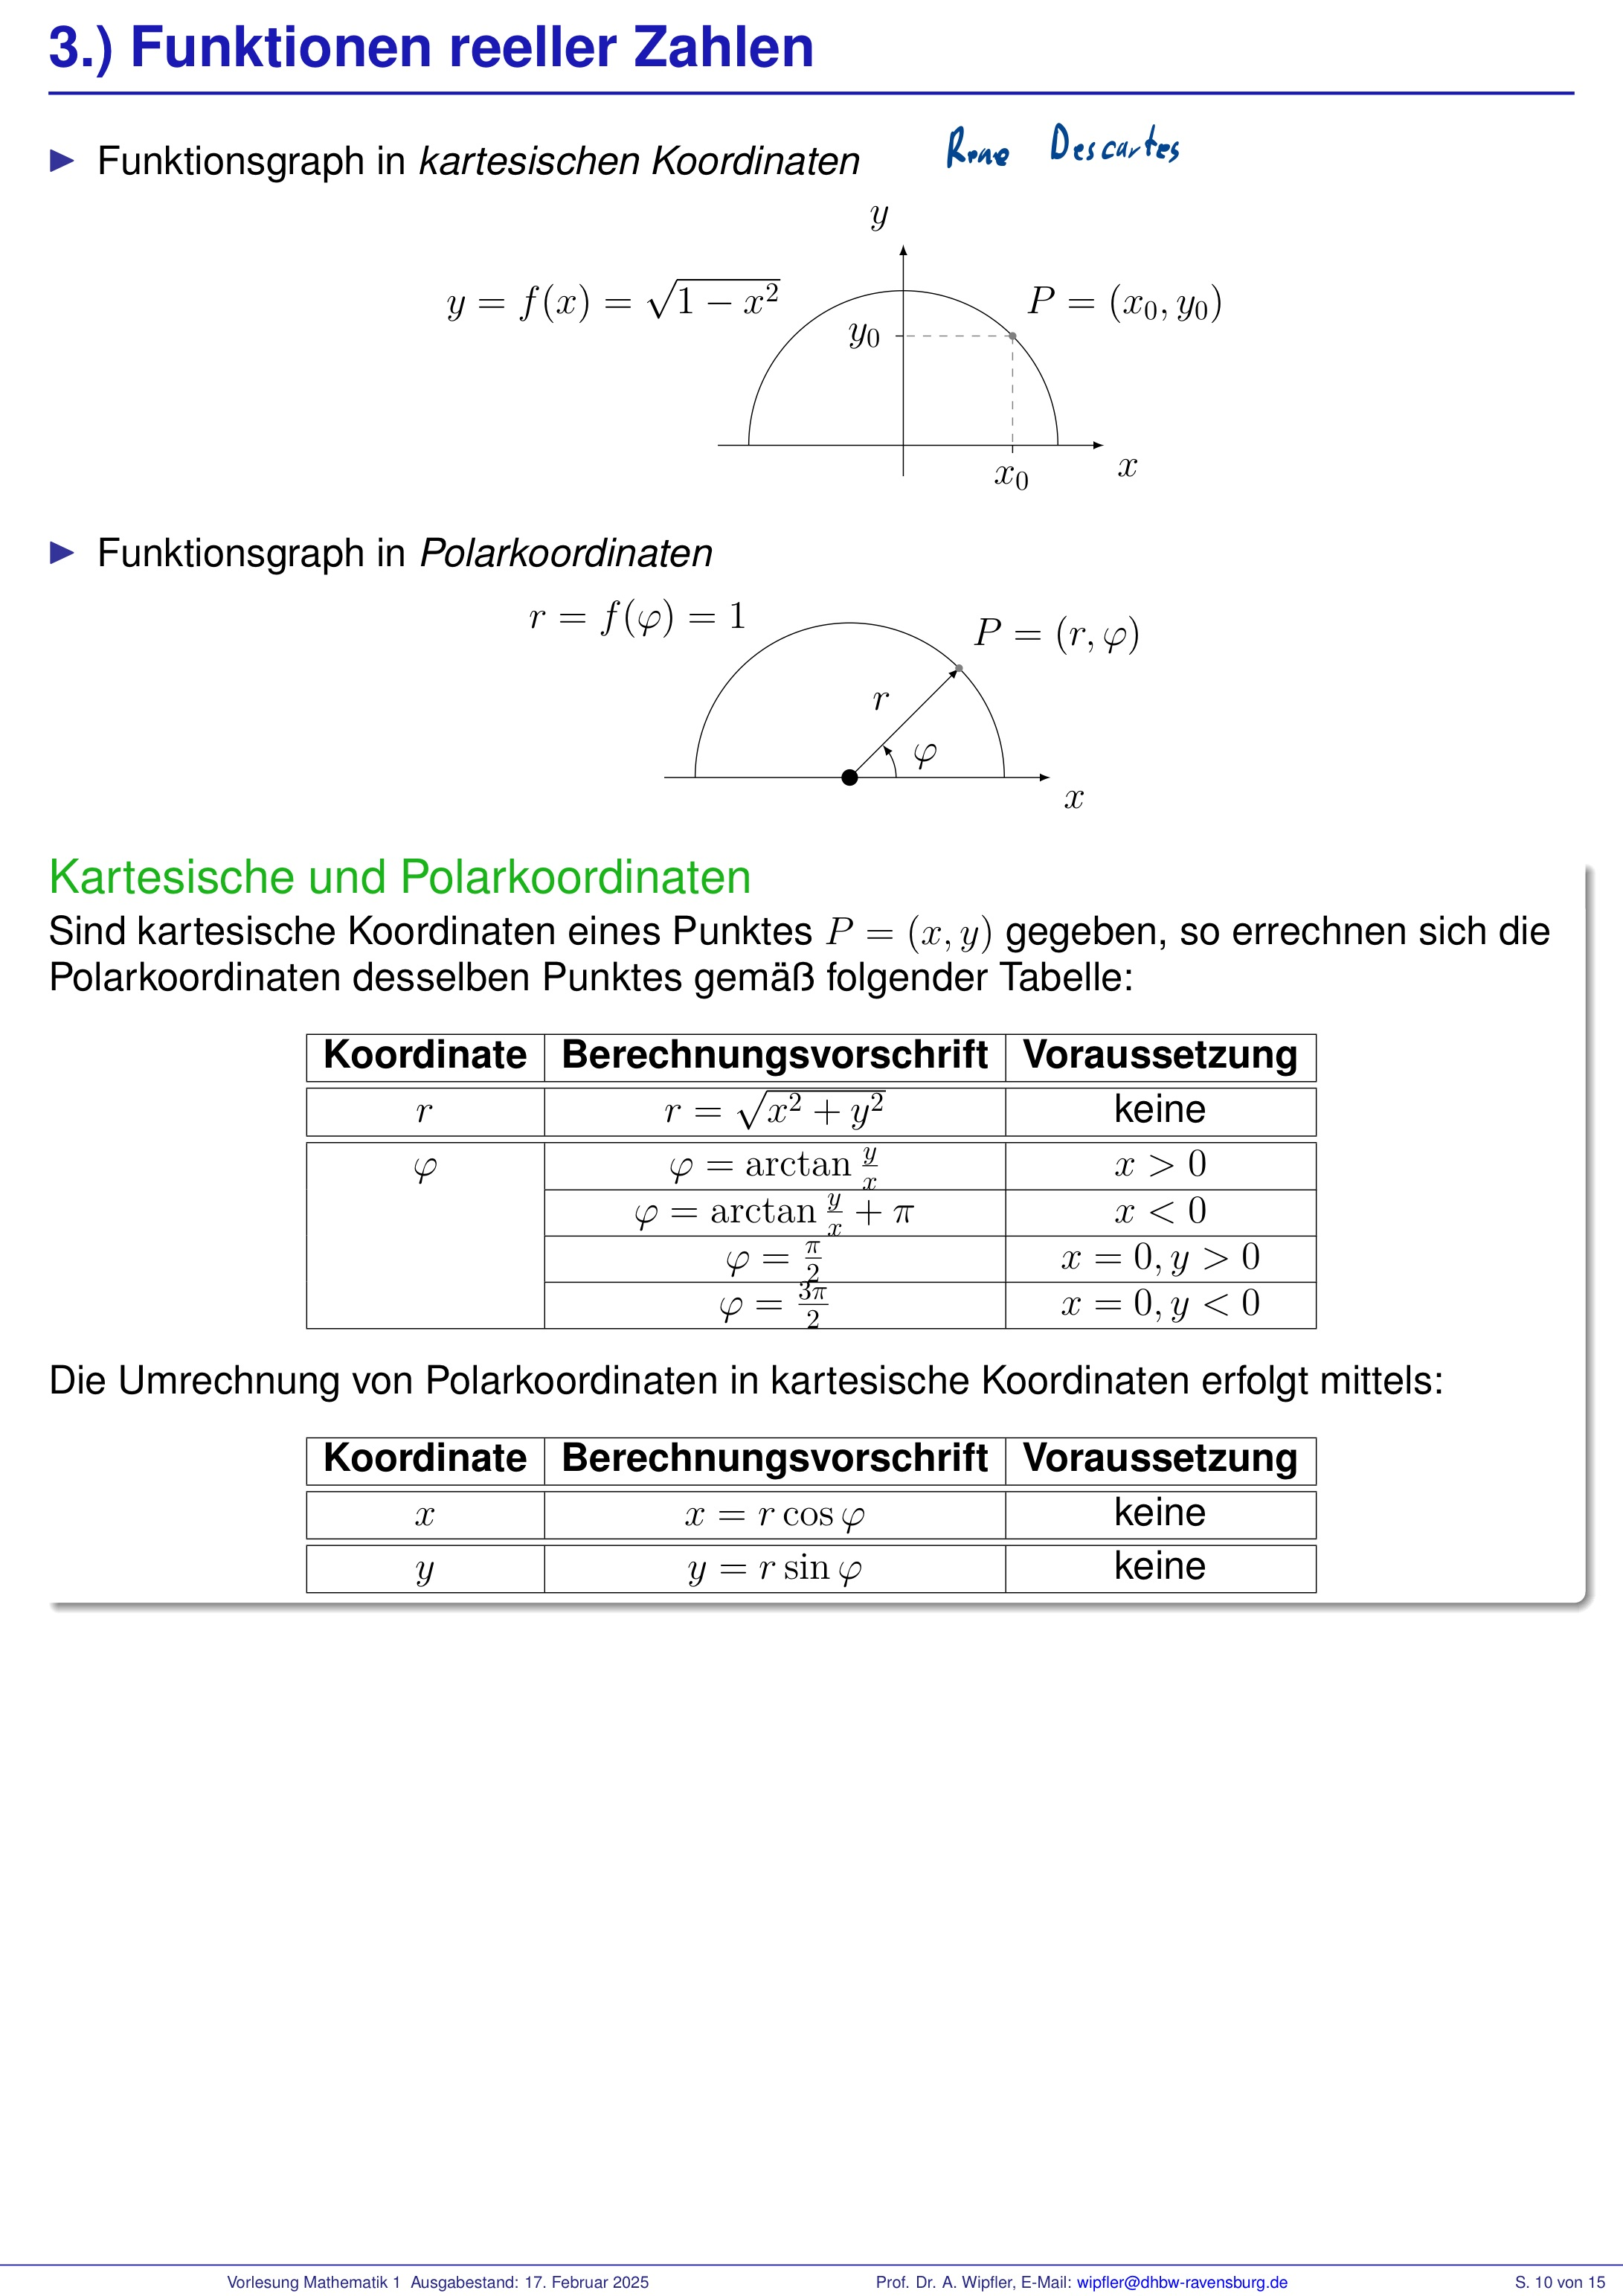
\includegraphics[width=0.7\textwidth]{KoordinatenUmrechnen-13} 
    \caption{Umrechnen von Koordinaten}
    \label{fig:komplexe_ebene}
\end{figure}

\newpage
\begin{tabular}{@{} l l @{}}

Admittanz & $\underline{Y} = \dfrac{1}{\underline{Z}}$ \\
\hspace*{20mm} Komplexer Leitwert & $\underline{Y} = G + jB$ \\
\end{tabular}

\vspace*{10mm}

Viele Regeln der Linearen Schaltungsanalysen gelten auch für komplexe Größen, z.B.: \\
\begin{tabular}{@{} l l @{}}
\hspace*{20mm} Spannungsteiler & $\underline{U}_1 = \underline{U} \cdot \dfrac{\underline{Z}_1}{\underline{Z}_1 + \underline{Z}_2}$ \\
\hspace*{20mm} Stromteiler & $\underline{I}_1 = \underline{I} \cdot \dfrac{\underline{Z}_2}{\underline{Z}_1 + \underline{Z}_2}$ \\
\hspace*{20mm} Ohmsches Gesetz & $\underline{U} = \underline{Z} \cdot \underline{I}$ \\
Stern-Dreick-Umwandlung & $\underline{Z}_1 = \dfrac{\underline{Z}_{12} \cdot \underline{Z}_{31}}{\underline{Z}_{12} + \underline{Z}_{23} + \underline{Z}_{31}}$ \\
& $\underline{Z}_2 = \dfrac{\underline{Z}_{12} \cdot \underline{Z}_{23}}{\underline{Z}_{12} + \underline{Z}_{23} + \underline{Z}_{31}}$ \\
& $\underline{Z}_3 = \dfrac{\underline{Z}_{13} \cdot \underline{Z}_{23}}{\underline{Z}_{12} + \underline{Z}_{23} + \underline{Z}_{31}}$ \\

Dreick-Stern-Umwandlung & $\underline{Z}_{12} = \underline{Z}_{1} + \underline{Z}_{2} + \dfrac{\underline{Z}_1 \cdot \underline{Z}_2}{\underline{Z}_3}$ \\
& $\underline{Z}_{23} = \underline{Z}_{2} + \underline{Z}_{3} + \dfrac{\underline{Z}_2 \cdot \underline{Z}_3}{\underline{Z}_1}$ \\
& $\underline{Z}_{31} = \underline{Z}_{3} + \underline{Z}_{1} + \dfrac{\underline{Z}_3 \cdot \underline{Z}_1}{\underline{Z}_2}$ \\  
\end{tabular}

Impedanzen in Reihen oder Parallel Anordnung werden berechnet wie reelle Widerstände: \\


\vspace*{10mm}
\noindent
\begin{minipage}{\textwidth}
\centering
Umwandlung RL-Serie in RL-Parallel\\[2mm]
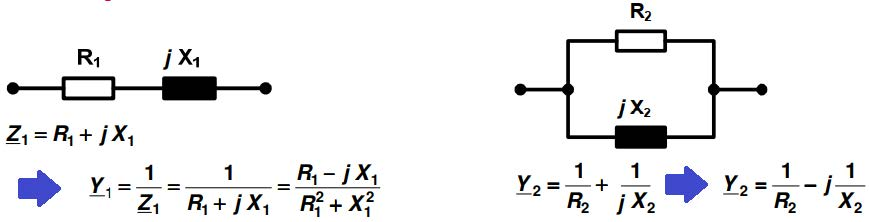
\includegraphics[width=0.7\textwidth]{Bild-FS1-RL-Serie-Umwandeln}
\end{minipage}

\vspace*{5mm}
\begin{tabular}{@{} l l @{}}

$R_2 = \dfrac{R_1^2 + X_1^2}{R_1}$ & $X_2 = \dfrac{R_1^2 + X_1^2}{X_1}$ \\

\end{tabular}

\vspace*{10mm}
\noindent
\begin{minipage}{\textwidth}
\centering
Umwandlung RL-Parallel in RL-Serie\\[2mm]
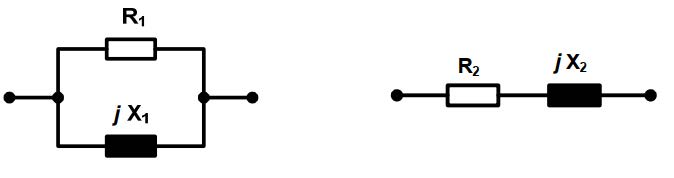
\includegraphics[width=0.7\textwidth]{Bild-FS1-RL-Parallel-Umwandeln}
\end{minipage}

\vspace*{5mm}
\begin{tabular}{@{} l l @{}}

$R_2 = R_1 \cdot \dfrac{X_1^2}{R_1^2 + X_1^2}$ & $X_2 = X_1 \cdot \dfrac{R_1^2}{R_1^2 + X_1^2}$ \\

Diese Formeln gelten auch für die Umwandlung von RC-Schaltungen, & \\
wobei dann folgendes eingesetzt werden muss & $X_1 = \dfrac{1}{\omega C_1}$ \\

\end{tabular}

Bei Schaltungen mit mehreren Quellen und unterschiedlichen Frequenzen addierung der Ergebnisse erst im Zeitbereich.

\newpage
\section{Foliensatz 2}

\begin{tabular}{@{} l l @{}}

\hspace*{20mm} Scheinleistung & $S= U_L \cdot I_L$ \\
\hspace*{20mm} Scheinleistung mit Phasor & $\underline{S}= P_W + j \cdot P_B$ \\
\hspace*{20mm} Wirkleistung & $P_w = S \cdot \cos \varphi $ \\
\hspace*{20mm} Blindleistung & $P_b = S \cdot \sin \varphi$ \\
\hspace*{20mm} Leistunggsfaktor & $\cos \varphi$ \\

\end{tabular}
\subsection{Leistung an einem Widerstand}
\begin{tabular}{@{} l l @{}}
\hspace*{20mm} Wirkleistung am Widerstand& $P_W = S = U \cdot I = \dfrac{U^2}{R}$ \\
Am Widerstand fällt keine Bildleistung am $\rightarrow$ Kein Imaginärteil \\

\end{tabular}

\subsection{Leistung an der Spule}
\begin{tabular}{@{} l l @{}}
  \hspace*{20mm} Scheinleistung an der Spule & $S= U \cdot I = \dfrac{U^2}{\omega L}>0$ \\
\end{tabular}

\subsection{Leistung an dem Kondensator}
\begin{tabular}{@{} l l @{}}
  \hspace*{20mm} Scheinleistung an einem Kondensator & $S=  -U \cdot I = -\omega C \cdot U^2<0$ \\
\end{tabular}

\subsection{Leistung der Komplexen Wechselspannung}
\begin{minipage}{\textwidth}
\centering
Leistung der Komplexen Wechselspannung\\[2mm]
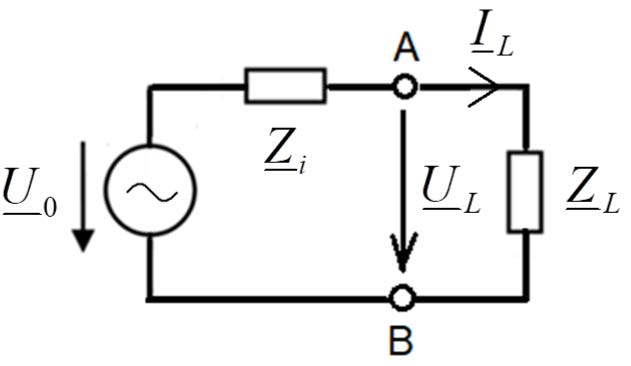
\includegraphics[width=0.7\textwidth]{Bild-FS2-Leistung-Komplexer-AC}
\end{minipage}


\begin{tabular}{@{} l l @{}}
\hspace*{20mm} Wirkleistung & $P_W = Re(\underline{S}) = Re(\underline{U}_L \cdot \underline{I}_L^*)= \lvert \underline{I}_L \rvert^2 \cdot Re(\underline{Z}_L) = I_L^2 \cdot Re(\underline{Z}_L)$ \\
 & $P_W = Re(\underline{S}) = Re(\underline{U}_L \cdot \underline{I}_L^*)= \lvert \underline{U}_L \rvert^2 \cdot Re(\underline{Y}_L) = U_L^2 \cdot Re(\underline{Y}_L)$ \\

 \hspace{20mm} Blindleistung & $P_B = Im(\underline{S}) = Im(\underline{U}_L \cdot \underline{I}_L^*)= \lvert \underline{I}_L \rvert^2 \cdot Im(\underline{Z}_L) = I_L^2 \cdot Im(\underline{Z}_L)$ \\
 & $P_B = Im(\underline{S}) = Im(\underline{U}_L \cdot \underline{I}_L^*)= \lvert \underline{U}_L \rvert^2 \cdot Im(\underline{Y}_L^*) = U_L^2 \cdot Im(\underline{Z}_L^*t)$ \\
\end{tabular}

\color{red}
\vspace*{5mm}
LEISTUNGSABPASSUNG NACHARBEITEN
\color{black}

\subsection{Schwingkreise}
RLC Serienschwingkreis

\begin{tabular}{@{} l l @{}}
\hspace*{20mm} Resonanzfrequenz & $\omega_0 = \dfrac{1}{\sqrt{L \cdot C}}$ \\
\hspace{20mm} Resonanzblindwiderstand & $X= \omega_0 \cdot L = \dfrac{1}{\sqrt{L \cdot C}} \cdot L = \sqrt{\dfrac{L}{C}}$ \\
\hspace*{20mm} Güte des Serienschwingkreises & $Q = \dfrac{X}{R} = \dfrac{\omega_0 \cdot L}{R}$ \\

\hspace*{20mm} Bei  $\dfrac{\omega}{\omega_0} = 0$ (DC Fall) gilt: & Reellwerige Spannung $U_C =$ Spannung $U_0$ \\

\hspace{20mm} RLC Impedanz & $\underline{Z}_{ges} = R + j \omega L + \dfrac{1}{j \omega C} = R + j \cdot \left( \omega L - \dfrac{1}{\omega C} \right)$ \\
Imaginärteil fällt weg bei: & $Im(\underline{Z}_{ges}) = 0$ für $\dfrac{\omega}{\omega_0}=1$ \\

Betrag der Impedanz wird minimiert  & Es gilt: $\lvert \underline{Z}_{ges} \rvert_{min} = R$ \\
\hspace{20mm} Es folgt für I (Strom) & $\lvert \underline{I} \rvert = \dfrac{\lvert \underline{U_0} \rvert}{\lvert \underline{Z}_{ges} \rvert_{min}} = \dfrac{U_0}{R}$ \\

Amplitudengang des Stroms & $ \lvert \underline{I} \rvert = \dfrac{\underline{U_0}}{\underline{Z_{ges}}} = \dfrac{U_0}{R \cdot \sqrt{1 + Q^2 \cdot \left( \dfrac{\omega}{\omega_0} - \dfrac{\omega_0}{\omega} \right)^2 }} $ \\

\vspace{5mm} & \\

GLC Parallelschwingkreis & \\

\hspace*{20mm} Resonanzfrequenz & $\omega_0 = \dfrac{1}{\sqrt{L \cdot C}}$ [wie bei RLC Serie]\\
\hspace{20mm} Resonanzblindwiderstand & $X= \omega_0 \cdot C = \dfrac{1}{\omega_0 \cdot L} = \sqrt{\dfrac{C}{L}}$ \\
\hspace*{20mm} Güte des Parallelschwingkreises & $Q = \dfrac{X}{G}$ \\
\hspace{20mm} GLC Admittanz & $\underline{Y}_{ges} = G + j \omega C + \dfrac{1}{j \omega L} = G + j \cdot \left( \omega C - \dfrac{1}{\omega L} \right)$ \\
Imaginärteil fällt weg bei: & $Im(\underline{Y}_{ges}) = 0$ für $\dfrac{\omega}{\omega_0}=1$ \\

\vspace{5mm} & \\
Bandbreite & $ B = f_2 - f_1 = \dfrac{f_0}{Q} $ \\
\end{tabular}


\subsection{Vierpole}

\begin{minipage}{\textwidth}
\centering
Beispiel Vierpol\\[2mm]
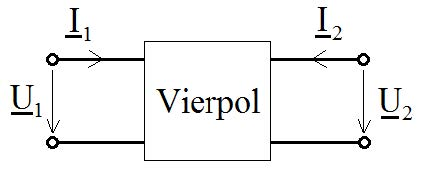
\includegraphics[width=0.7\textwidth]{Bild-FS2-Vierpole1}
\end{minipage}

\begin{tabular}{@{} l l @{}}
Spannungen & $\underline{U}_1 = \underline{Z}_{11} \cdot \underline{I}_1 + \underline{Z}_{12} \cdot \underline{I}_2$ \\
& $\underline{U}_2 = \underline{Z}_{21} \cdot \underline{I}_1 + \underline{Z}_{22} \cdot \underline{I}_2$ \\

Impedanzen (z-Parameter)& \\
\hspace{20mm} Eingangsimpedanz & $\underline{Z}_{11} = \dfrac{\underline{U}_1}{\underline{I}_1} \bigg|_{\underline{I}_2=0}$ \\
\hspace{20mm} Vorwärts Transimpedanz & $\underline{Z}_{21} = \dfrac{\underline{U}_2}{\underline{I}_1} \bigg|_{\underline{I}_2=0}$ \\
\hspace{20mm} Rückwärts Transimpedanz & $\underline{Z}_{12} = \dfrac{\underline{U}_1}{\underline{I}_2} \bigg|_{\underline{I}_1=0}$ \\
\hspace{20mm} Ausgangsimpedanz & $\underline{Z}_{22} = \dfrac{\underline{U}_2}{\underline{I}_2} \bigg|_{\underline{I}_1=0}$ \\

Ströme & $\underline{I}_1 = \underline{Y}_{11} \cdot \underline{U}_1 + \underline{Y}_{12} \cdot \underline{U}_2$ \\
& $\underline{I}_2 = \underline{Y}_{21} \cdot \underline{U}_1 + \underline{Y}_{22} \cdot \underline{U}_2$ \\

Admittanzen Kurzschluss (y-Parameter) & \\
\hspace{20mm} Eingangsadmittanz & $\underline{Y}_{11} = \dfrac{\underline{I}_1}{\underline{U}_1} \bigg|_{\underline{U}_2=0}$ \\
\hspace{20mm} Vorwärts Kernadmittanz & $\underline{Y}_{21} = \dfrac{\underline{I}_2}{\underline{U}_1} \bigg|_{\underline{U}_2=0}$ \\
\hspace{20mm} Rückwärts Kernadmittanz & $\underline{Y}_{12} = \dfrac{\underline{I}_1}{\underline{U}_2} \bigg|_{\underline{U}_1=0}$ \\
\hspace{20mm} Ausgangsadmittanz & $\underline{Y}_{22} = \dfrac{\underline{I}_2}{\underline{U}_2} \bigg|_{\underline{U}_1=0}$ \\

Hybride Formen & \\
Spannungen & $\underline{U}_1 = \underline{h}_{11} \cdot \underline{I}_1 + \underline{h}_{12} \cdot \underline{u}_2$ \\
Strom & $\underline{I}_2 = \underline{h}_{21} \cdot \underline{I}_1 + \underline{h}_{22} \cdot \underline{u}_2$ \\
Hybride Parameter (h-Parameter) & \\
 & $\underline{h}_{11} = \dfrac{\underline{U}_1}{\underline{I}_1} \bigg|_{\underline{u}_2=0}$ \\
 & $\underline{h}_{12} = \dfrac{\underline{U}_1}{\underline{u}_2} \bigg|_{\underline{I}_1=0}$ \\
 & $\underline{h}_{21} = \dfrac{\underline{I}_2}{\underline{I}_1} \bigg|_{\underline{U}_2=0}$ \\
 & $\underline{h}_{22} = \dfrac{\underline{U}_2}{\underline{I}_2} \bigg|_{\underline{I}_1=0}$ \\

\end{tabular}


\begin{tabular}{@{} l l @{}}
  Spannung & $\underline{U}_2 = \underline{k}_{21} \cdot \underline{U}_1 + \underline{k}_{22} \cdot \underline{I}_2$ \\
  Strom & $\underline{I}_1 = \underline{k}_{11} \cdot \underline{U}_1 + \underline{k}_{12} \cdot \underline{I}_2$ \\

Hybride Parameter (k-Parameter / P-Parameter) & \\
 & $\underline{k}_{11} = \dfrac{\underline{I}_1}{\underline{U}_1} \bigg|_{\underline{I}_2=0}$ \\
 & $\underline{k}_{12} = \dfrac{\underline{I}_1}{\underline{I}_2} \bigg|_{\underline{U}_1=0}$ \\
 & $\underline{k}_{21} = \dfrac{\underline{U}_2}{\underline{U}_1} \bigg|_{\underline{I}_2=0}$ \\
 & $\underline{k}_{22} = \dfrac{\underline{U}_2}{\underline{I}_2} \bigg|_{\underline{U}_1=0}$ \\  


Spannung & $\underline{U}_1 = \underline{A}_{11} \cdot \underline{U}_2 + \underline{A}_{12} \cdot \underline{-I}_2$ \\
Strom & $\underline{I}_1 = \underline{A}_{21} \cdot \underline{U}_2 + \underline{A}_{22} \cdot \underline{-I}_2$ \\

 Kettenparameter (a-Parameter) & \\
 & $\underline{A}_{11} = \dfrac{\underline{U}_1}{\underline{U}_2} \bigg|_{\underline{I}_2=0}$ \\
 & $\underline{A}_{12} = \dfrac{\underline{U}_1}{\underline{-I}_2} \bigg|_{\underline{U}_2=0}$ \\
 & $\underline{A}_{21} = \dfrac{\underline{I}_1}{\underline{U}_2} \bigg|_{\underline{I}_2=0}$ \\
 & $\underline{A}_{22} = \dfrac{\underline{I}_1}{\underline{-I}_2} \bigg|_{\underline{U}_2=0}$ \\

Spannung & $\underline{U}_2 = \underline{B}_{11} \cdot \underline{U}_1 + \underline{B}_{12} \cdot \underline{I}_1$ \\
Strom & $\underline{-I}_2 = \underline{B}_{21} \cdot \underline{U}_1 + \underline{B}_{22} \cdot \underline{I}_1$ \\

 Kettenparameter (B-Parameter) & \\
 & $\underline{B}_{11} = \dfrac{\underline{U}_2}{\underline{U}_1} \bigg|_{\underline{I}_1=0}$ \\
 & $\underline{B}_{12} = \dfrac{\underline{U}_2}{\underline{I}_1} \bigg|_{\underline{U}_1=0}$ \\
 & $\underline{B}_{21} = \dfrac{\underline{-I}_2}{\underline{U}_1} \bigg|_{\underline{I}_1=0}$ \\
 & $\underline{B}_{22} = \dfrac{\underline{-I}_2}{\underline{I}_1} \bigg|_{\underline{U}_1=0}$ \\

\end{tabular}

%Einfügen der Bilder 4-Pol 2,3. weitermachen bei FS-2 seite 80

\end{document}